% Copyright (c) 2013,  Lawrence Livermore National Security, LLC.
% Produced at the Lawrence Livermore National Laboratory.
% This file is part of WARP.  See file COPYRIGHT for details.

% WARP is free software; you can redistribute it and/or modify it under the
% terms of the GNU Lesser General Public License (as published by the Free
% Software Foundation) version 2.1 dated February 1999.

% Latex header for doxygen 1.8.5
\documentclass[twoside]{article}

% Packages required by doxygen
\usepackage{calc}
\usepackage{localdoxygen}
\usepackage{graphicx}
\usepackage[utf8]{inputenc}
\usepackage{makeidx}
\usepackage{multicol}
\usepackage{multirow}
\usepackage{textcomp}
\usepackage[table]{xcolor}

% Font selection
\usepackage[T1]{fontenc}
\usepackage{mathptmx}
\usepackage[scaled=.90]{helvet}
\usepackage{courier}
\usepackage{amssymb}
\usepackage{sectsty}
\renewcommand{\familydefault}{\sfdefault}
\allsectionsfont{%
  \fontseries{bc}\selectfont%
  \color{darkgray}%
}
\renewcommand{\DoxyLabelFont}{%
  \fontseries{bc}\selectfont%
  \color{darkgray}%
}

% Page & text layout
\usepackage{geometry}
\geometry{%
  letterpaper,%
  top=1in,%
  bottom=1in,%
  left=1in,%
  right=1in%
}
\tolerance=750
\hfuzz=15pt
\hbadness=750
\setlength{\emergencystretch}{15pt}
\setlength{\parindent}{0cm}
\setlength{\parskip}{0.2cm}
\makeatletter
\renewcommand{\paragraph}{% To remove paragraph numbers, set the 4 to 8
  \@startsection{paragraph}{4}{0ex}{-1.0ex}{1.0ex}{%
    \normalfont\normalsize\bfseries\SS@parafont%
  }%
}
\renewcommand{\subparagraph}{%
  \@startsection{subparagraph}{5}{0ex}{-1.0ex}{1.0ex}{%
    \normalfont\normalsize\bfseries\SS@subparafont%
  }%
}
\makeatother

% Headers & footers
\usepackage{fancyhdr}
\pagestyle{fancyplain}
\fancyhead[LE]{\fancyplain{}{\bfseries\thepage}}
\fancyhead[CE]{\fancyplain{}{}}
\fancyhead[RE]{\fancyplain{}{\bfseries\leftmark}}
\fancyhead[LO]{\fancyplain{}{\bfseries\rightmark}}
\fancyhead[CO]{\fancyplain{}{}}
\fancyhead[RO]{\fancyplain{}{\bfseries\thepage}}
\fancyfoot[LE]{\fancyplain{}{}}
\fancyfoot[CE]{\fancyplain{}{}}
\fancyfoot[RE]{\fancyplain{}{\bfseries\scriptsize Generated on Tue Nov 12 2013 12\-:07\-:46 for warp by Doxygen }}
\fancyfoot[LO]{\fancyplain{}{\bfseries\scriptsize Generated on Tue Nov 12 2013 12\-:07\-:46 for warp by Doxygen }}
\fancyfoot[CO]{\fancyplain{}{}}
\fancyfoot[RO]{\fancyplain{}{}}
\renewcommand{\footrulewidth}{0.4pt}
\renewcommand{\sectionmark}[1]{%
  \markright{\thesection\ #1}%
}

% Indices & bibliography
\usepackage{natbib}
\usepackage[titles]{tocloft}
\setcounter{tocdepth}{3}
\setcounter{secnumdepth}{5}
\makeindex

% Packages requested by user
\usepackage{amsmath,amsfonts,amssymb}

% Hyperlinks (required, but should be loaded last)
\usepackage{ifpdf}
\ifpdf
  \usepackage[pdftex,pagebackref=true]{hyperref}
\else
  \usepackage[ps2pdf,pagebackref=true]{hyperref}
\fi
\hypersetup{%
  colorlinks=true,%
  linkcolor=blue,%
  citecolor=blue,%
  unicode%
}

% Subfloat
\usepackage[caption = false]{subfig}

% Custom commands
\newcommand{\clearemptydoublepage}{%
  \newpage{\pagestyle{empty}\cleardoublepage}%
}
\def\XVec#1{{\mathbf #1}}       
\def\XOne{{\mathbf 1}}          
\def\XFGrid{{\cal G}}           
\def\XCGrid{{\cal G}_c}                                         
\def\XReals{{\mathbb R}}
\def\XFSpace{\XReals^{n}}       
\def\XCSpace{\XReals^{n_c}}     
\def\XSSpace{\XReals^{n_s}}     
\def\XFPts{{\cal F}}            % set of C pts
\def\XCPts{{\cal C}}            % set of F pts
\def\XNPts{{\cal N}}            % set of neighbor pts
\def\XPx{P_{\star}}
\def\Xu{\XVec{u}}
\def\Xf{\XVec{f}}
\def\Xg{\XVec{g}}              
\def\Xe{\XVec{e}}
\def\Xr{\XVec{r}}
\def\Xx{\XVec{x}}
\def\Xy{\XVec{y}}
\def\Xv{\XVec{v}}
\def\Xw{\XVec{w}}
\def\XUnit{\mbox{\boldmath $\varepsilon$}}  
\def\XCL{{\cal L}}
\def\XCM{{\cal M}}
\def\Xux{\boldsymbol{u}}
\def\Xfx{\boldsymbol{f}}
\def\Xgx{\boldsymbol{g}}


%===== C O N T E N T S =====

\begin{document}

% Titlepage & ToC
\hypersetup{pageanchor=false}
\pagenumbering{roman}
\begin{titlepage}

~\\~\\~\\~\\
\begin{tabular*}{6.5in}{l@{\extracolsep{\fill}} l}
\multirow{2}{*}{{\huge Developers' Manual} }   & {\Large Version 1.0} \\
                                               & {\Large \today} \\
\end{tabular*}
\rule{\textwidth}{3pt}
~\\~\\~\\~\\~\\~\\~\\
\begin{figure}[!ht]
     \centering
     
\includegraphics[width=0.35\textwidth]{../img/warp.pdf}
\end{figure}
~\\
\begin{figure}[!ht]
     \centering
     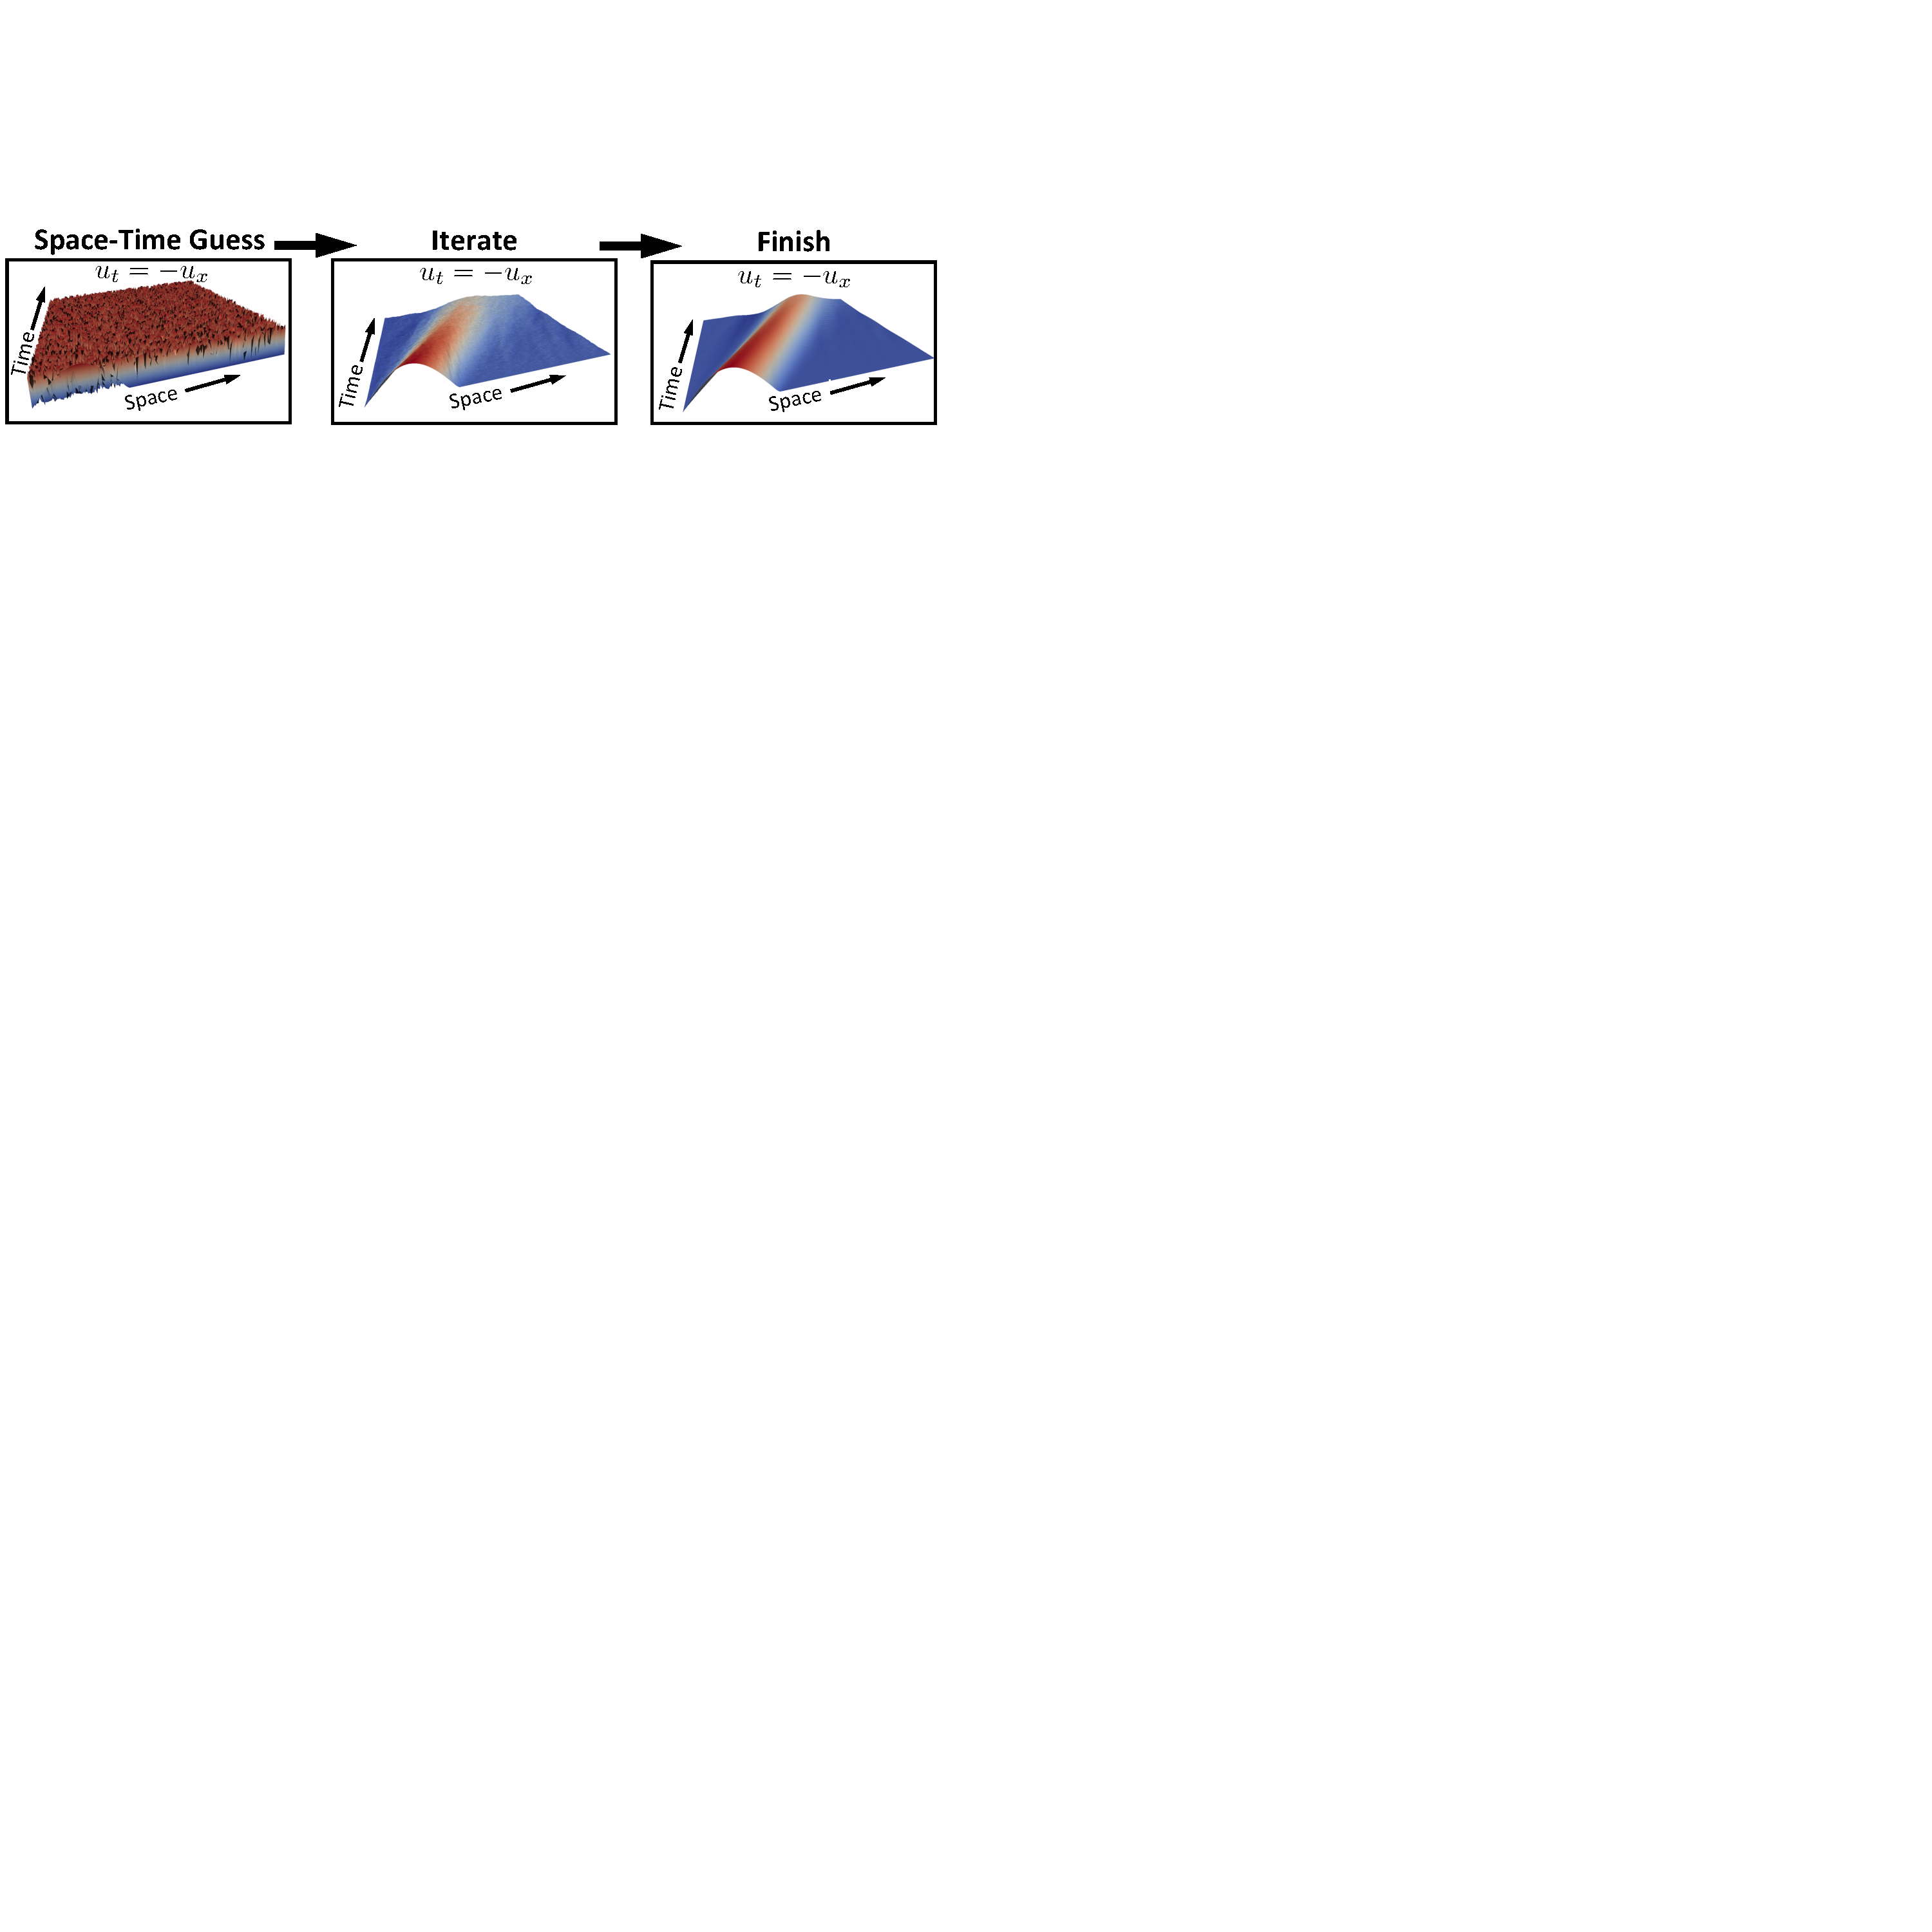
\includegraphics[width=0.8\textwidth]{../img/title.pdf}
\end{figure}

~\\~\\~\\~\\~\\~\\~\\~\\~\\~\\~\\~\\~\\~\\~\\~\\
\begin{tabular*}{6.5in}{l@{\extracolsep{\fill}} l}
 V.~A. Dobrev, R.~D. Falgout, Tz.~V. Kolev, N.~A. Petersson, J.~B. Schroder, U.~M. Yang  & \\
 Center for Applied Scientific Computing (CASC)  &  \\
 Lawrence Livermore National Laboratory          &  \\
\end{tabular*}
\rule{\textwidth}{2pt}
~\\
This work performed under the auspices of the U.S. Department of Energy by
Lawrence Livermore National Laboratory under Contract DE-AC52-07NA27344.
LLNL-******
\pagebreak

Copyright (c) 2013,  Lawrence Livermore National Security, LLC.
Produced at the Lawrence Livermore National Laboratory.
Written by the WARP team.  All rights reserved.
~\\~\\ 
This file is part of WARP. Please see the COPYRIGHT and LICENSE file 
for the copyright notice, disclaimer, contact information and the 
GNU Lesser General Public License.
~\\~\\
WARP is free software; you can redistribute it and/or modify it under the
terms of the GNU General Public License (as published by the Free Software
Foundation) version 2.1 dated February 1999.
~\\~\\
WARP is distributed in the hope that it will be useful, but WITHOUT ANY
WARRANTY; without even the IMPLIED WARRANTY OF MERCHANTABILITY or FITNESS FOR A
PARTICULAR PURPOSE. See the terms and conditions of the GNU General Public
License for more details.
~\\~\\
You should have received a copy of the GNU Lesser General Public License along
with this program; if not, write to the Free Software Foundation, Inc., 59
Temple Place, Suite 330, Boston, MA 02111- 1307 USA

\end{titlepage}
\tableofcontents
\pagenumbering{arabic}
\hypersetup{pageanchor=true}

%--- Begin generated contents ---
